\section{Introduction}
\subsection{Purpose}

The purpose of this document is to present a detailed description of our Final Year Project, InstaWeight. It will explain the purpose and features of the system, the core components and the interface of the system. It will give in-depth information of our system that we will developed. 

\subsection{Scope}
The aim of the system is to estimate the weight of the cattle accurately. The system is designed to automate the process of measuring cattle’s weight on a large scale in a farm. Moreover, it will keep track of the daily growth of the cattle’s weight to take decisions related to live stock business. The core component of the system will be responsible to detect the features of the animal from the image to estimate/predict the weight of the animal. This core component will be developed using machine learning and image processing algorithms. 

\vspace*{2mm} On client side, there will be a admin panel to the store the weight of cattle and see the growth trend of each cattle. The system will also contain a relational database containing the basic information such as id, age, gender, weight etc. of each cattle. 

\subsection{Overview of the document}
The next section of this document, ‘the overall description’ gives an overview of the functionality of the system. It describes the functional and non-functional requirements, use case diagrams, system diagram and external interfaces. 

\section{Overall Description}

\subsection{System Environment}

The autonomous weight estimating system has two active actors a system with three components. A normal user/ farmer can capture the image of a cattle to measure the weight of an animal. The camera would be connected to the core component of the system. The weight would be saved in admin panel. The owner of the farm or a rancher can access the admin panel to keep track of the growth of the cattle.\\



\begin{figure}[h]
\centering
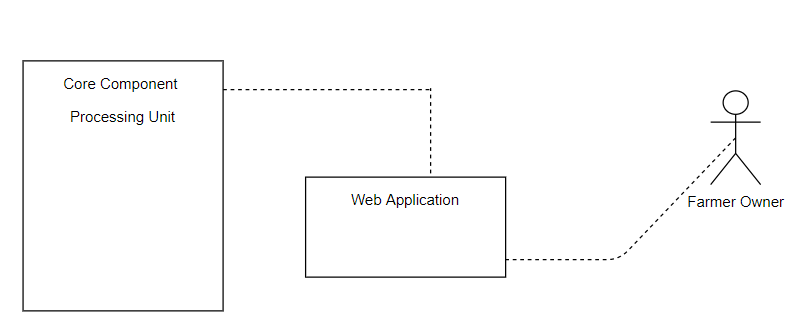
\includegraphics [scale=0.6] {ed.png}
\caption{System Environment Diagram}
\end{figure}


\pagebreak

\section{Functional Requirements}

\subsection{Business Requirements}

\begin{enumerate}
\item The system should be 90\% to 95\% accurate.
\end{enumerate}

\subsection{Web Application (Admin Panel):}

	The core functionalities of admin panel would be following: 
\begin{enumerate}
	\item \textbf{Authentication:}
	\begin{enumerate}
		\item The sign up of all users would be done by the admin panel. 
		\begin{enumerate}
			\item To sign up into the system, the basic information of the user would be required and will be added to the system. 
		\end{enumerate}
	\end{enumerate}

	\item \textbf{Dashboard:}
\begin{enumerate}
	\item The admin panel would display the overall growth of all cattle in last six months through pi-chart. 
	\item It would show the growth progress of each cattle on individual level in last six months. 
	\item Admin panel would have different tabs and button to add, update and delete.
	  \item Record of the animal can be update by clicking on the “Update Record” tab. 
	 \item The cattle’s record can be deleted by “Delete” button. 
\end{enumerate}

	\item \textbf{Cattle Management: }
	
	\begin{enumerate}
		\item \textbf{Add Cattle}
		\begin{enumerate}
			\item To add an animal into the system, it would be required to add some details such as age, gender, type etc. into the system.
		\end{enumerate}
		\item \textbf{List View}
		\begin{enumerate}
			\item List of all animals would be displayed.
		\end{enumerate}
		\item \textbf{View Details}
		\begin{enumerate}
			\item On clicking view details, the complete details of every individual animal would be displayed on screen. 
		\end{enumerate}
\end{enumerate}
	
	\item \textbf{Under Observation:}
	\begin{enumerate}
		\item All cattle who are diagnosed ill or under stress by the system and needs checkup. 
	\end{enumerate}
	
	\item \textbf{Settings:}
	\begin{enumerate}
		\item Personal configuration section from where admin can change password and other login details. 
	\end{enumerate}
	
\end{enumerate}



% --- The above is to be modified as per your project, e.g. a flat list if your system has limited functional requirements.

\section{Non-functional Requirements}

\hspace*{10mm} Following are the non-functional requirements of our system. 
\begin{enumerate}
	\item \textbf{Security:}\\
	The user's data that would be required during sign up should be confidential, safe and secure.
	\item \textbf{Performance:}\\
	The system should less than a minutes to process the image and estimate weight.
	\item \textbf{Compatible:}\\
	The system should be compatible with all android devices. 
	\item \textbf{Memory Efficient:}\\
	The mobile application should be space efficient and should not occupy large space of memory.
	\item \textbf{Usability:}
	The interface of the system should be simple and flow of app should be understandable by farmer who is not well educated. 
	\item \textbf{Scalability:}\\
	The system should be scalable so that it can later be used in real world or at industry level. 
	\item \textbf{Maintainability:}
	The system should be easily maintainable so that it can become more advance and efficient when use in industry. 
	\item \textbf{Legal:}\\
	According to the intellectual property rights, the system should only be used by Folio3. 
	
\end{enumerate}

\pagebreak
\section{External Interfaces}

\subsection{User Interfaces}
\subsubsection{Admin Dashboard}

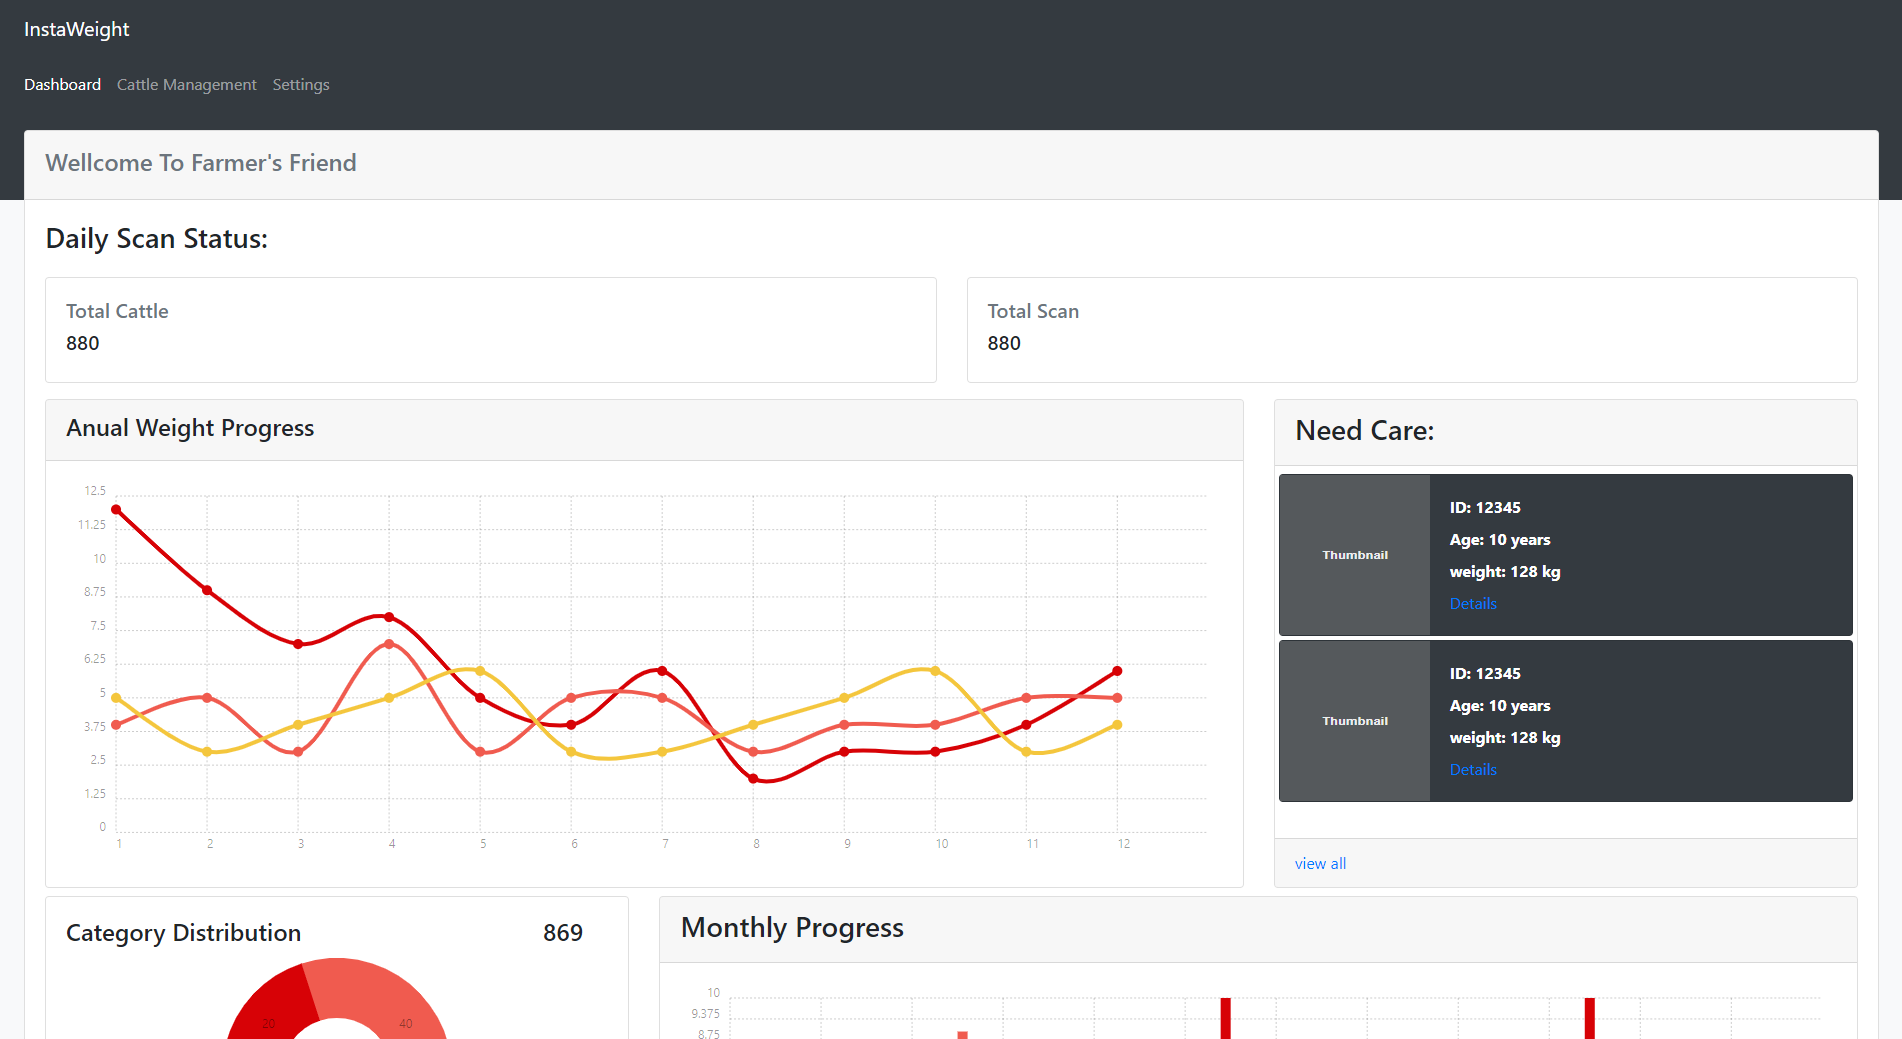
\includegraphics [scale=0.3] {dashboard-1half.png}

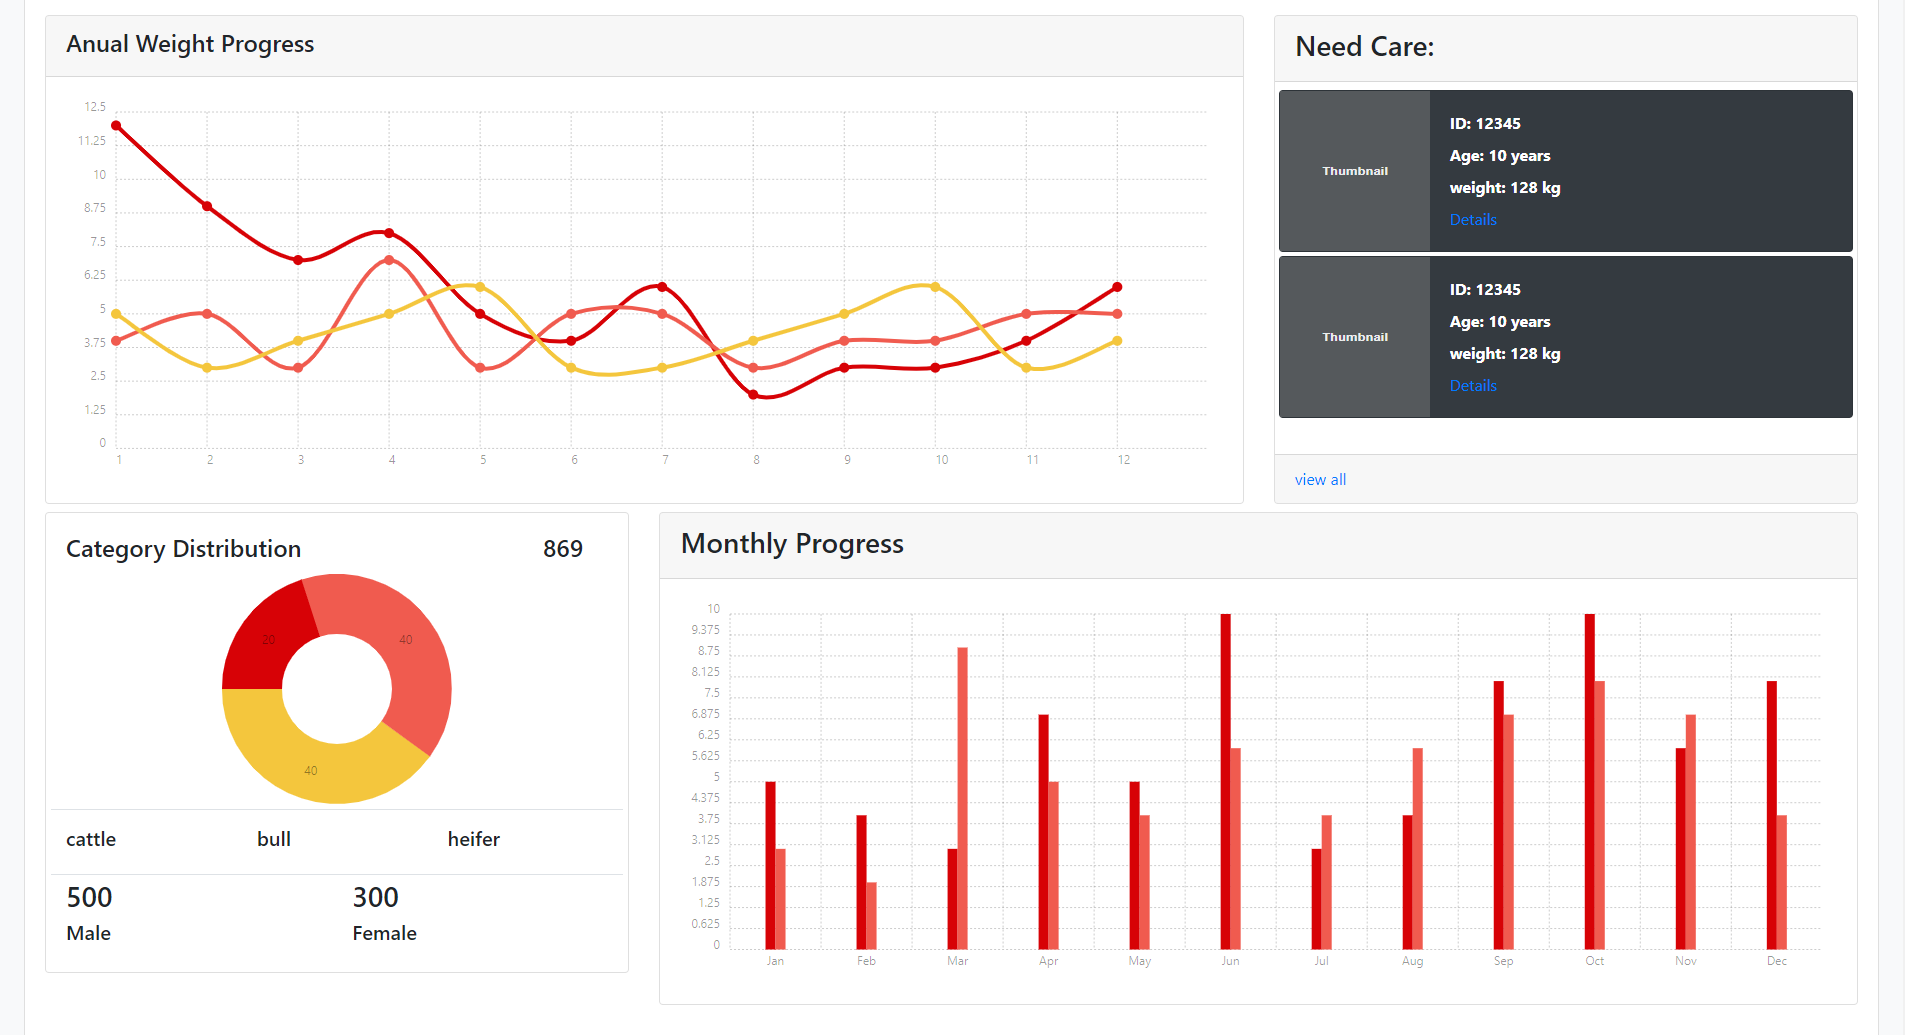
\includegraphics [scale=0.3] {dashboard-2half.png} \\

This page will display some graphes which will show annual and monthly animals' progress. it will also display animal which need special care. 

\newpage
\subsection{Cattle Management:}

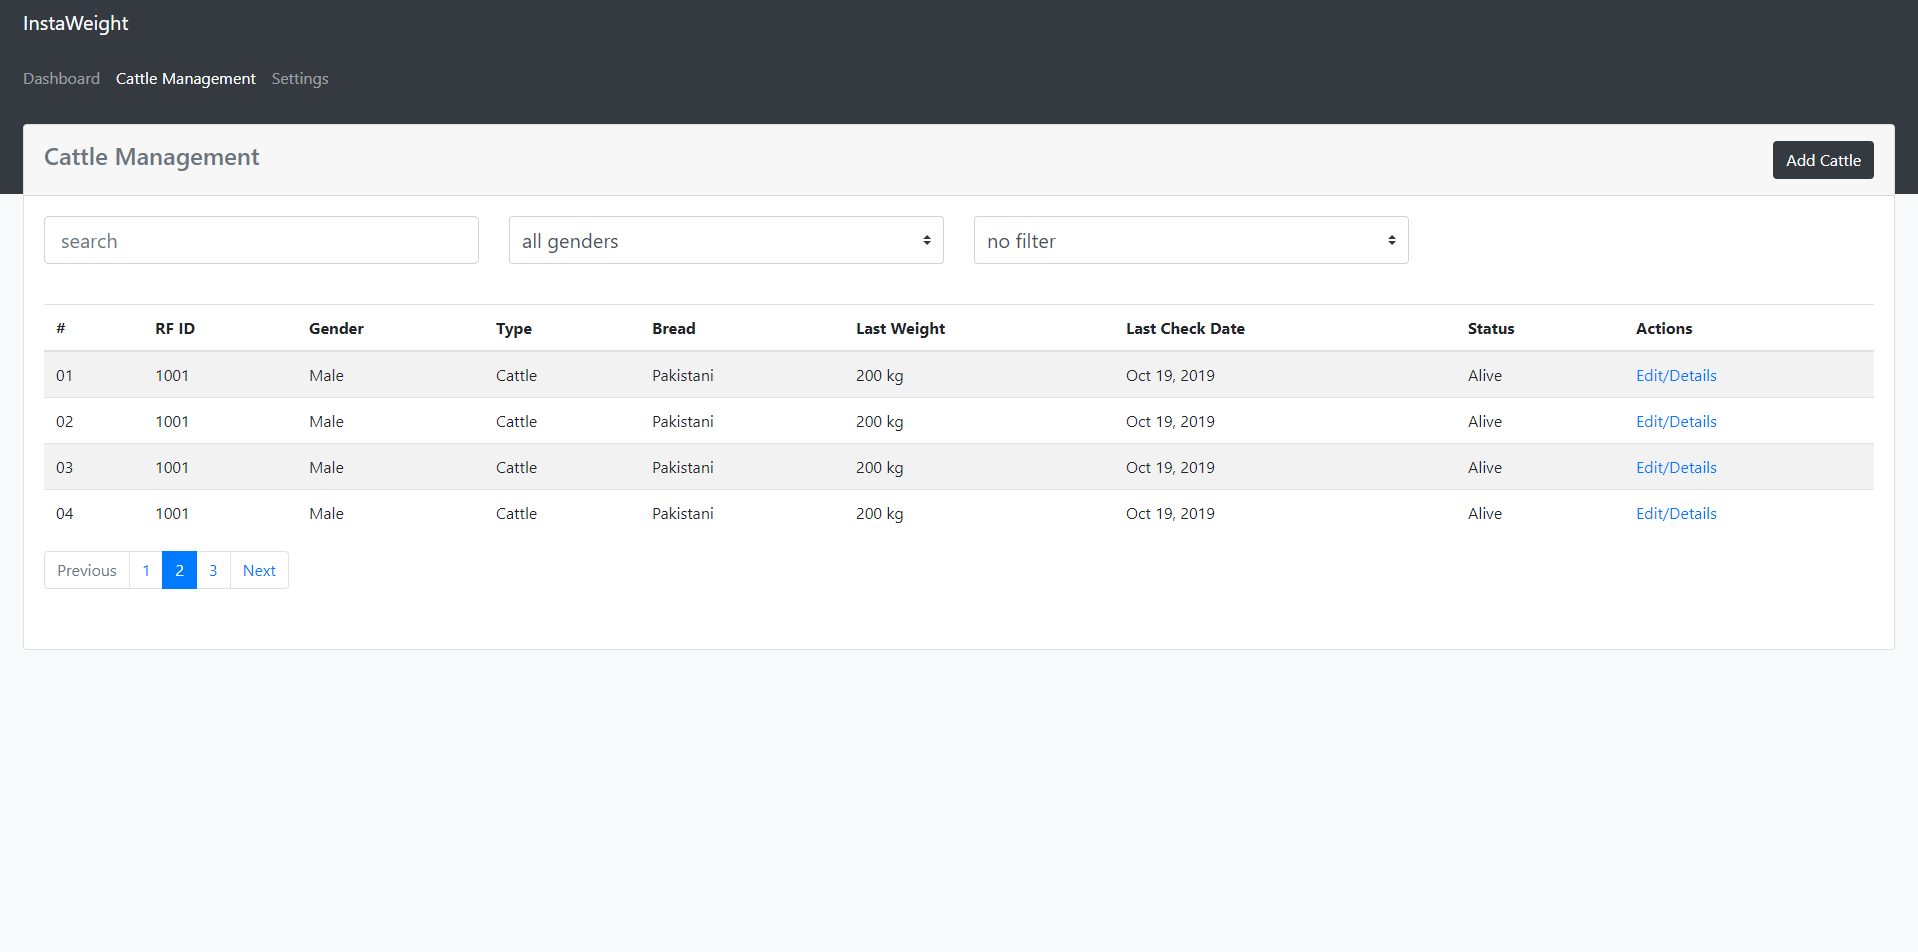
\includegraphics [scale=0.3] {cattle-management.png} \\

This will display all animals in a tabular form and will let user filter the animals and see their details.

\newpage

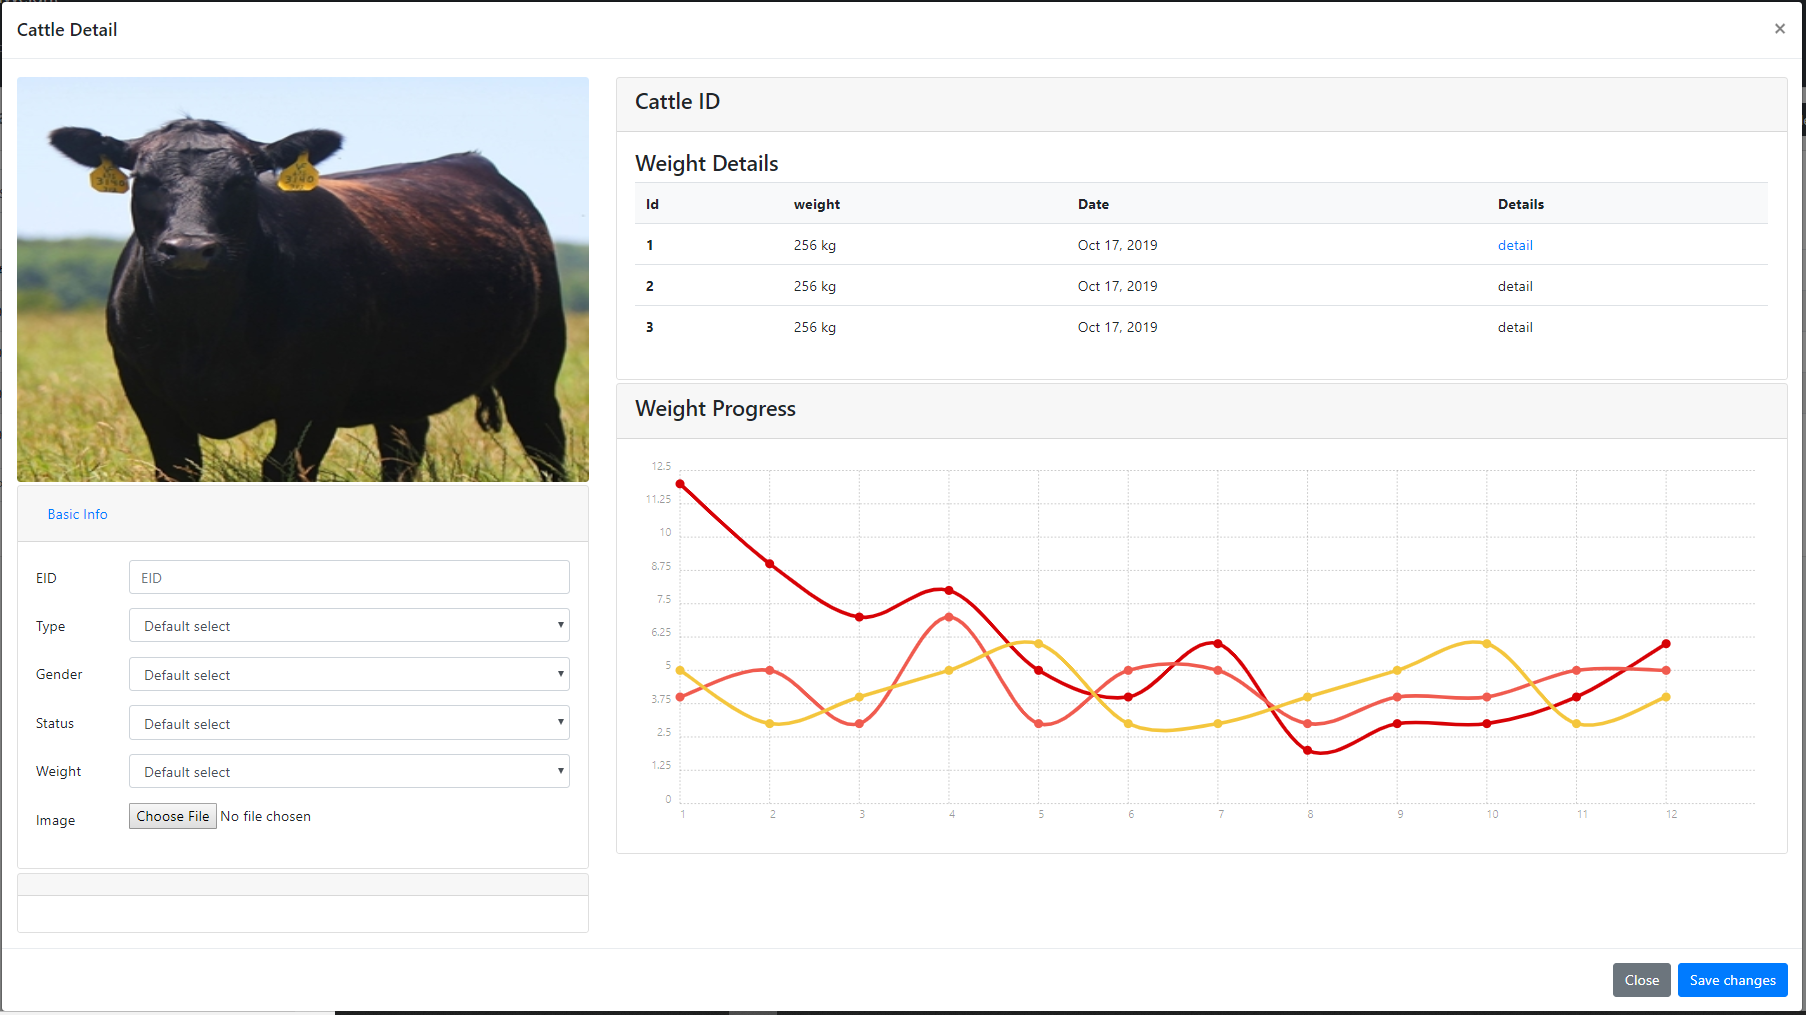
\includegraphics [scale=0.3] {details-modal.png} \\

This will display details of a single cattle and lets user edit it.

\newpage

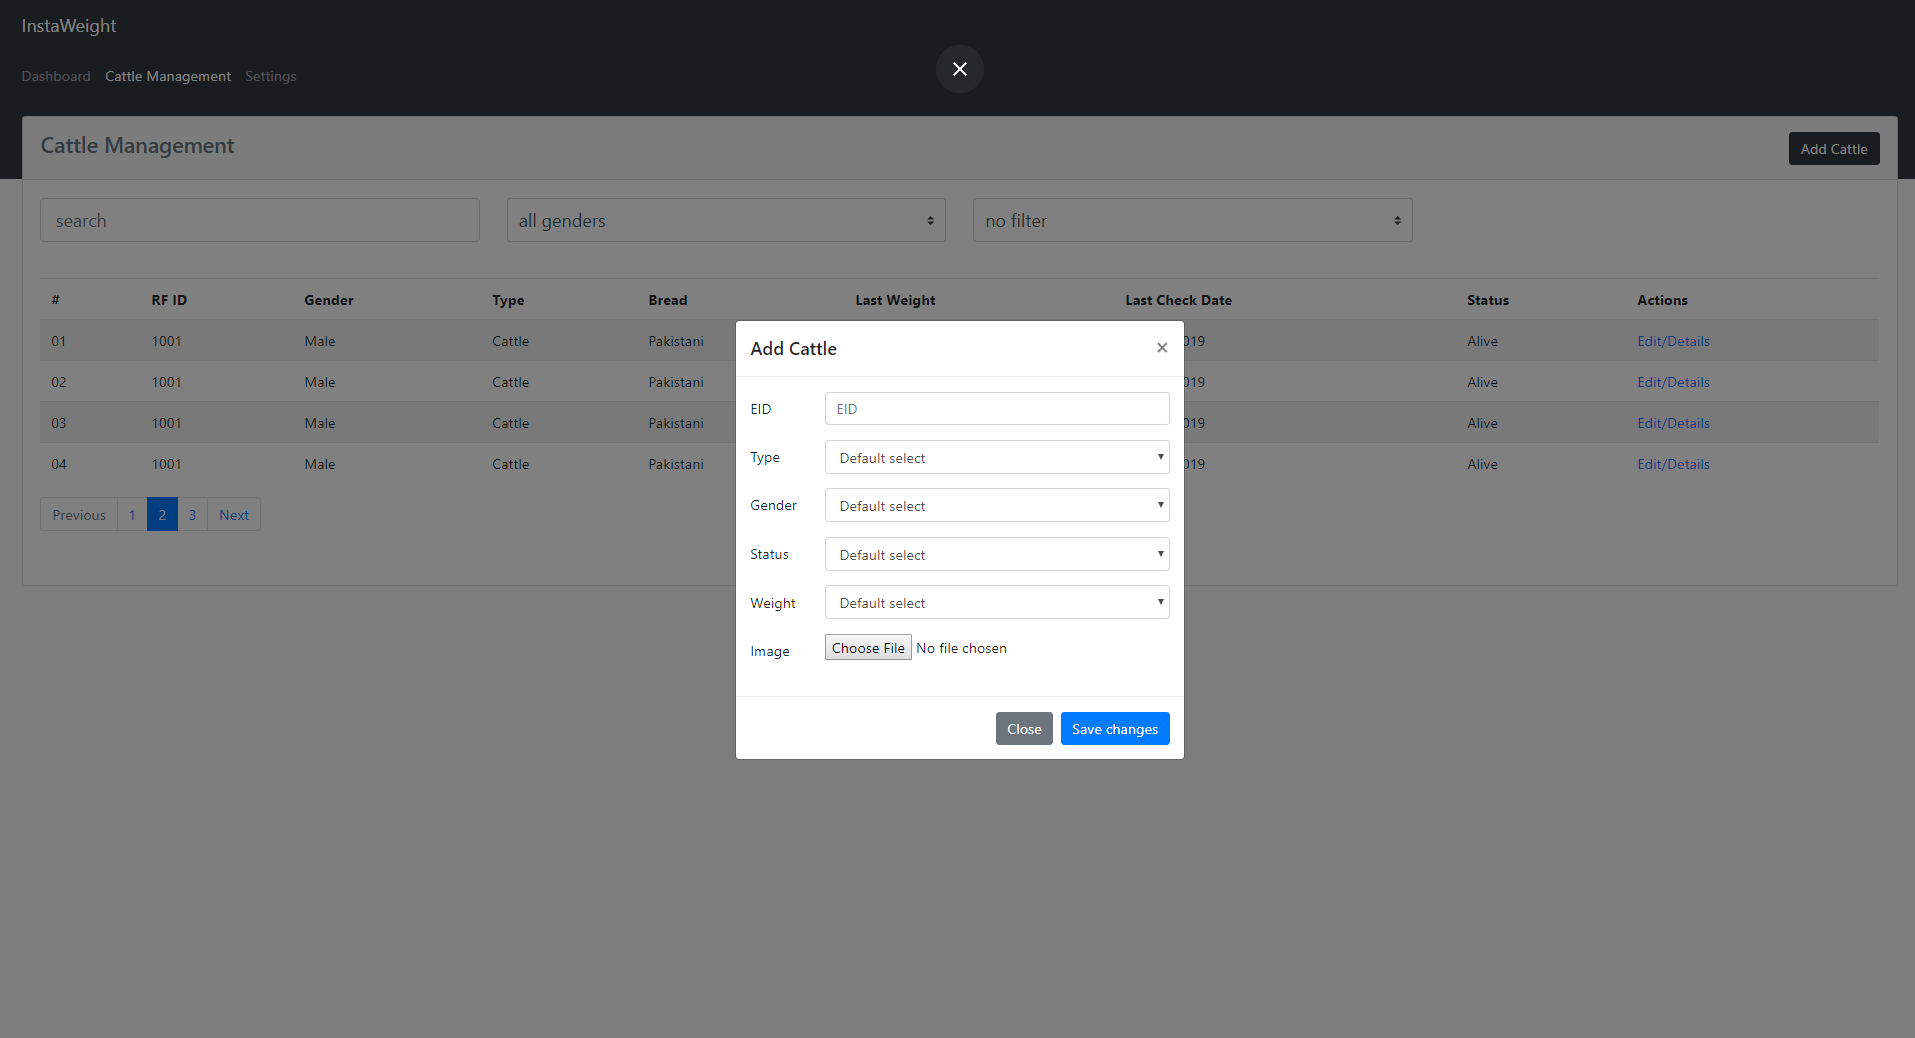
\includegraphics [scale=0.3] {add-cattle-modal.png} \\

This will will be the interface though which a new cattle can be added details of a single cattle and lets user edit it.

\newpage

\subsection{Dataset and Augmentation}
\subsubsection{Dataset Collection:}

The dataset was collected 3 times. Here are the details of the dataset:
\begin{enumerate}
\item \textbf{Dataset V1} - This dataset was collected on a farm having about 150 animals and approximately 1200 RGB images were collected. All of the dataset was annotated for two bounding boxes, one to enclose the whole cattle (outer bounding box) and the other to enclose abdomen of the cattle (inner bounding box). Out of those 1200 images 229 were usable. We also scrapped about 700 images from google and around 277 were usable. These images only consisted of a side view of the Cattle and no depth and weight labels were available. These images were used for inner and outer bounding box detection. We augmented this dataset by making each image brightened with gamma = 2.0. We then darkened the image and introduced noise to simulate low light conditions. The images were flipped on a vertical axes. hence generated 3 augmented images out of one. The total number of images after augmentation were about 2,024.
\begin{figure}[h]
\centering
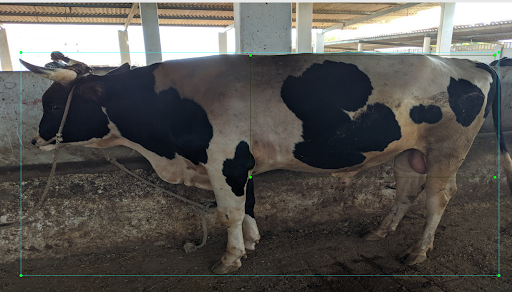
\includegraphics[scale=0.5]{datasetv1.jpg}
\caption{Annotation on V1 for inner and outer bounding box}
\end{figure}


\item \textbf{Dataset V2} - This dataset was collected on a farm having about 65 animals. Approximately 1235 RGB images with depth were taken. We annotated these images for the Inner and outer boxes as well as for Semantic Segmentation. These were also side views of the cattle and no informatio of cattle's weight was available. Total images in our dataset were 1235 with depth, 229 (original from V1 without depth) and 2,024 (including original, augmented and scraped images) without depth. These images were used for Semantic Segmentation and bounding boxes. 
\pagebreak 
\begin{figure}[h]
\centering
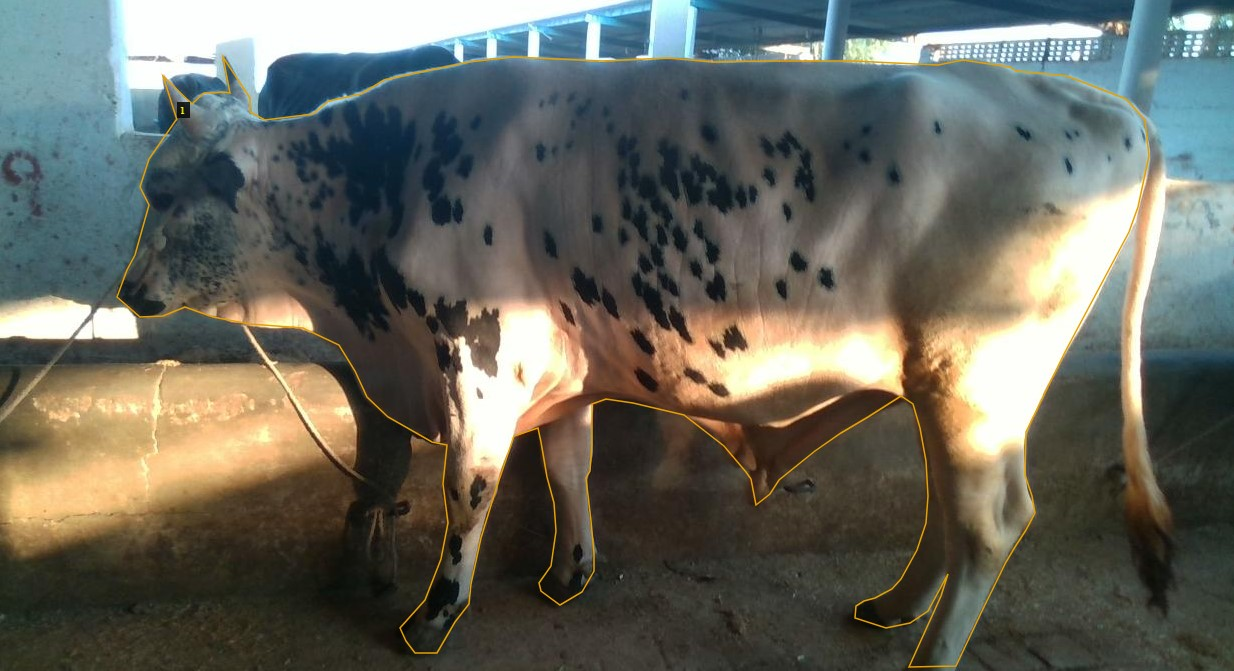
\includegraphics[scale=0.3]{maskRCNNAnnotation.jpg}
\caption{Annotation on V2 for mask RCNN}
\end{figure} 
\\

\item  \textbf{Dataset V3} - This dataset was taken urgently and only 8 animals were available. This dataset was created because the previous image with depth has some noise in depth values and a lot of zero values appear in the depth. The problem aroused because the camera was not calibrated correctly. After correct calibration, Approximately \textbf{1000} RGB images with Depth were taken. This dataset was also annotated for inner and outer rectangles but was only used for depth reated experiments. 


\end{enumerate}
\textbf{All of these images were annotated by our own team. We were unable to get cattle's weight labeled dataset because most of the farms do not keep it. And due to Covid-19 we were unable to make any further progress regarding data collection.}

\pagebreak
\section{System Diagram}
This diagram gives a high-level view of the different components of our system and the interactions between them. Each component and the particular tools/technologies/libraries used to build it are described.


\begin{figure}[h]
\centering
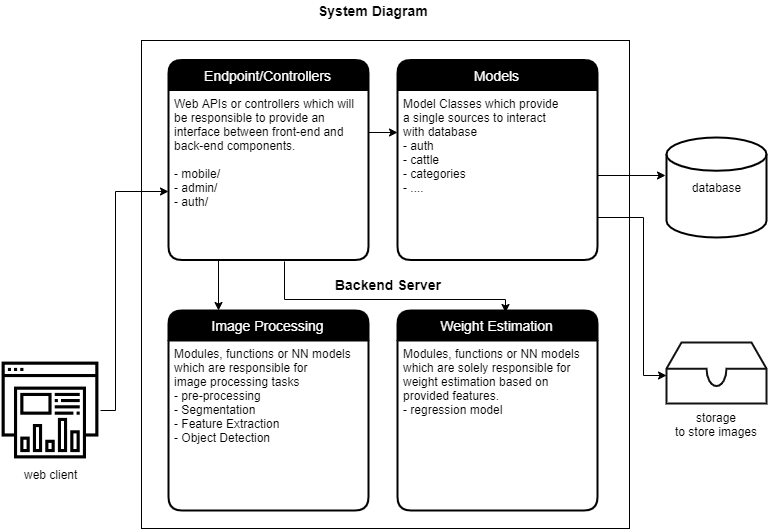
\includegraphics [scale=0.5] {system}
\caption{System Diagram}
\end{figure}


\subsection{Database}
This component will be responsible of storing data into relational format. This will be only accessible by Models (in MVC) component in the back-end. \\  \\
\textbf{Tools and Technologies: } PostgreSQL, SQL.\\

\subsection{Back-end Server}
This component will have further subcomponents:
\begin{enumerate}
\item \textbf{Models:}
This component is responsible to defining the schema of the database and interact with the database. This is the only module which interacts with the database, so that there is one source of truth for insertion and retrival of data. 
\item  \textbf{Image Processing module:}
This component will have methods responsible for segmentation, object detection and features extraction. 
\item \textbf{Weight Estimation:}
		Modules, functions or NN models which are solely responsible for weight estimation based on provided features. 		\\ i.e. regression model

\item \textbf{Endpoints / controllers:}
These Endpoints will define communication routes between server and clients and will bridge between the frontend and backend components. \\
\end{enumerate}
Collectively we refer to \textbf{Image Processing} and \textbf{Weight Estimation} as  \textbf{Core}. \\ \\
\textbf{Tools/Technologies:} OpenCV, Django 2, MXnet, \\

\subsection{Webclient}
 This component will be helping in managing the information of animal and keeping tack of their weights on the go. \\
\textbf{Tools/Technologies:}
 Html, CSS, JavaScript


\pagebreak
\section{Architecture Diagram}

The following is the architecture diagram of the system which would be consists of four different layers. Since the system follow the MVC structure, these layers would be of view, controller, and model layers. There would be another layer of storage, which consists of database of the system. Layers are in hierarchical order, it means that every layer can communicate with its neighbour only. 


\begin{figure}[h]
\centering
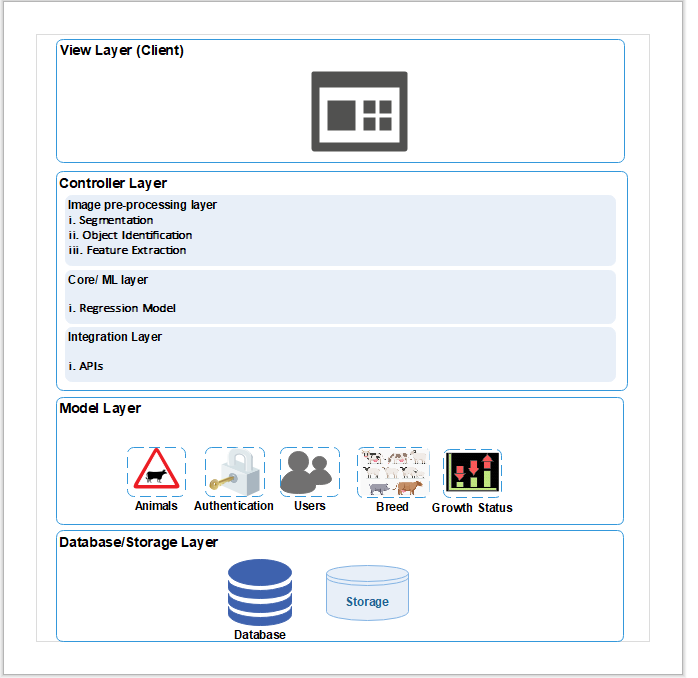
\includegraphics [scale=0.5] {ad.jpg}
\caption{Architecture Diagram}
\end{figure}


\pagebreak 
\section{Use Cases}

This section presents detailed use cases of our system.This diagram illustrates the basic breakdown of our system in terms of use cases and actors. The expanded use cases are provided ahead. 
\begin{figure}[h]
\centering
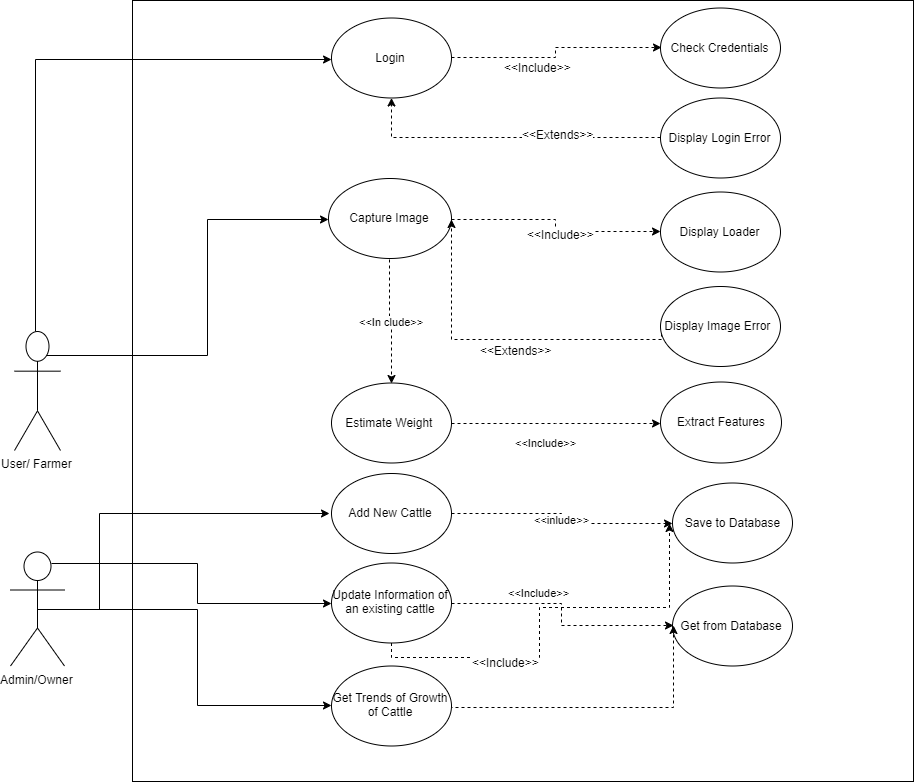
\includegraphics [scale=0.4] {uc}
\caption{Use Case Diagram}
\end{figure}



\pagebreak

\textbf{Use Case 1: Login}

\begin{tabular}{|l|p{.60\textwidth}|p{0.30\textwidth}|}
	\hline
	Use-Case Name: & Login\\ \hline
	Use-Case ID:& UC-01 \\\hline
	Priority:& High\\ \hline
	Source:& None \\ \hline
	Primary Business Actor: & User/Client\\ \hline
	Other Participating Actors:&  No one\\ \hline
	Description:&  The user would login the application as well as admin panel to use the system. Only authenticated users will be allowed to login. \\ \hline
	Precondition:&  User must be registered. \\ \hline
	Trigger:&  When user enters his credentials and clicks on submit. \\ \hline 
	Typical course of events:&  \textbf{Actor Action:}
	\begin{enumerate}
		\item 	User enters the credentials and clicks on submit button.
	\end{enumerate}

	\vspace{2mm}
	
	\textbf{System Action: }
	\begin{enumerate}
		\item System checks the credentials of the user and validate them.
		\item 	If the credentials are valid. User is allowed to use the system, else error generated. 
	\end{enumerate}
	\\ \hline
	Conclusion:  & If credentials are valid, them user will logged in.\\ \hline
	Post Condition: & None \\ \hline
\end{tabular}\\
\\


\pagebreak

\textbf{Use Case 2: Capture Images}

\begin{tabular}{|l|p{.60\textwidth}|p{0.15\textwidth}|}
	\hline
	Use-Case Name: & Capture Images\\ \hline
	Use-Case ID:& UC-02 \\\hline
	Priority:& High\\ \hline
	Source:& None \\ \hline
	Primary Business Actor: & User/Client\\ \hline
	Other Participating Actors:&  No one\\ \hline
	Description:&  The user would capture the image of a cattle from front and side view. The images would be captured from a particular angle and only two images would be captured. \\ \hline
	Precondition:&  User must be authenticated. \\ \hline
	Trigger:&  When user is logged in into the system and click on the camera button to capture the image.  \\ \hline 
	Typical course of events:&  \textbf{Actor Action:}
	\begin{enumerate}
		\item The actor clicks on the button to capture image. 
		
	\end{enumerate}
	\vspace{2mm}
	
	\textbf{System Action: }
	\begin{enumerate}
		\item	After capturing the image, the image is sent to server for further processing.  
		
	\end{enumerate}
	\\ \hline
	Conclusion:  & The image is captured by the mobile application at a certain angle and sent to server for further processing. \\ \hline
	Post Condition: & The image is sent to the server  for further processing.  \\ \hline
\end{tabular}\\


\pagebreak

\textbf{Use Case 3: Add New Cattle}\\


\begin{tabular}{|l|p{.60\textwidth}|p{0.15\textwidth}|}
	\hline
	Use-Case Name: & Add New Cattle\\ \hline
	Use-Case ID:& UC-05 \\\hline
	Priority:& High\\ \hline
	Source:& None \\ \hline
	Primary Business Actor: & Farm's owner/ Admin.\\ \hline
	Other Participating Actors:&  System/Admin Panel\\ \hline
	Description:& When new cattle is added in the farm, the basic details of the cattle such as age, gender, unique id is stored in the system’s database through admin panel \\ \hline
	Precondition:& User must be authenticated.   \\ \hline
	Trigger:& On clicking the “Add new cattle” button on admin panel.    \\ \hline 
	Typical course of events:&  \textbf{Actor Action:}
	\begin{enumerate}
		\item Admin click on “Add new cattle” tab and enters the information related to animal and click on the save button.  
	\end{enumerate}
	\textbf{System Action: }
	\begin{enumerate}
		\item 	System take those information and send it to database to save. 
	\end{enumerate}
	
	\\ \hline
	Conclusion:  & The record of the new cattle is saved into the database. \\ \hline
	Post Condition: &The information can be shown through admin panel.  \\ \hline
\end{tabular}\\


\pagebreak
\textbf{Use Case 4: Update Cattle Information into the Database}\\


\begin{tabular}{|l|p{.60\textwidth}|p{0.15\textwidth}|}
	\hline
	Use-Case Name: & Update cattle information into the database. \\ \hline
	Use-Case ID:& UC-06 \\\hline
	Priority:& High\\ \hline
	Source:& None \\ \hline
	Primary Business Actor: & Farm's owner/ Admin.\\ \hline
	Other Participating Actors:&  System/Admin Panel\\ \hline
	Description:& The cattle information can be updated by admin at any time when needed. The updated information will overwrite the previous information.  \\ \hline
	Precondition:& The cattle information is already added and saved in the system.    \\ \hline
	Trigger:& When information changes, the admin will update the information into the system.    \\ \hline 
	Typical course of events:&  \textbf{Actor Action:}
	\begin{enumerate}
		\item Admin click on “Update cattle info” tab and updates the information click on the save button.  
	\end{enumerate}
	\textbf{System Action: }
	\begin{enumerate}
		\item The system save the updated information into the database.
	\end{enumerate}
	
	\\ \hline
	Conclusion:  & The information is updated into the database.\\ \hline
	Post Condition: &The updated information is displayed through admin panel. \\ \hline
\end{tabular}\\


\pagebreak
\textbf{Use Case 5: Get Trends of Growth of Cattle}\\


\begin{tabular}{|l|p{.60\textwidth}|p{0.15\textwidth}|}
	\hline
	Use-Case Name: & Get trend of growth of cattle. \\ \hline
	Use-Case ID:& UC-07 \\\hline
	Priority:& High\\ \hline
	Source:& None \\ \hline
	Primary Business Actor: & Farm's owner/ Admin.\\ \hline
	Other Participating Actors:&  System/Admin Panel\\ \hline
	Description:& The cattle growth trend will be shown on admin panel on the basis of their weight estimated by the system. The trends will be shown on individual level. The pi-chart would also be displayed on panel to show the overall progress.  The system will display the last six months record.   \\ \hline
	Precondition:& The cattle information is already added and saved in the system.     \\ \hline
	Trigger:&It would be the core functionality of the admin panel and will be displayed by default on admin panel.     \\ \hline 
	Typical course of events:&  \textbf{Actor Action:}
	\begin{enumerate}
		\item No action would be done by user.  
	\end{enumerate}
	\textbf{System Action: }
	\begin{enumerate}
		\item The system will display the trends to show the growth progress. 
	\end{enumerate}
	
	\\ \hline
	Conclusion:  & The growth trends will be shown on the panel.\\ \hline
	Post Condition: &  The user can keep track of the animal’s weight of last six month. \\ \hline
\end{tabular}\\
